%!TEX root = ../main.tex


\section{Experiments}
\label{sec:experiments}

In this section, we carefully study the sensitivity of the
basic, optimized and incremental variations of the \sys algorithm 
to changes in the database and query log characteristics.
Due to the difficulty of collecting corrupt query logs from active deployments, 
our goal instead is to understand these trade-offs in
controlled synthetic scenarios, as well as use common OLTP query workloads
from two widely used database benchmarks.

To this end, we first focus on the case of single query corruptions and evaluate
the optimized \sys incremental algorithm on two OLTP benchmarks (Section~\ref{sec:experiments:benchmark}) and find that \sys can return high quality repairs in interactive speeds.
We then evaluate the variations of the incremental algorithm in a wide range of controlled database and query log settings (Section~\ref{sec:experiments:inc})
Finally, we evaluate the incremental and basic algorithms on more challenging settings of incomplete complaint sets and multiple query corruptions and discuss why the latter setting is fundamentally difficult (Section~\ref{sec:experiments:synth}).
All experiments were run on 12x2.66 GHz  machines with 16GB RAM running IBM CPLEX~\cite{cplex2014v12} as the MILP solver on CentOS release 6.6.
In the following text, \sys refers to the incremental algorithm with the tuple-slicing optimization: this setting works well in most OLTP benchmark settings because the tables
seldom have more than 50 attributes; Section~\ref{sec:experiments:dbproperties} shows how attribute and query-slicing can further improve performance an wide (up to $500$ attributes) tables.
We refer the reader to Appendix~\ref{sec:heuristic} for a study of alternative machine learning-based repair algorithms.

\iffalse
and to our full technical report~\cite{qfixarxiv} \alex{SIGMOD IS ANONYMOUS!} for an analysis of the MILP solver, factors that affect the 
number of complaints, and ambiguous repair situations (e.g., when multiple queries may be repaired to fix the complaint set).
\fi


% the performance and accuracy
% characteristics of the basic MILP-based repair algorithm, 
% slicing-based optimizations that improve the latency of the system, 
% and the incremental algorithm for single query corruptions. 

% \looseness -1
% \xlw{
% To this end, our experiments are organized as follows: First, 
% we compare the basic and incremental MILP algorithm against the different optimizations 
% to highlight the value of different optimizations and the limitations of the basic approach. We then evaluate \sys using established database transaction benchmarks from OLTP-bench~\cite{difallah2013oltp}:
% TPC-C~\cite{tpcc} and TATP~\cite{tatp}. In addition, we study the behavior of \sys using synthetic data sets and show that \texttt{UPDATE} queries are particularly difficult to repair and focus solely
% on different types of \texttt{UPDATE}-only workloads to understand how \sys responds to different parameter settings.
% We end with a discussion of \sys's capability in solving problems in more complex settings.}
% All experiments were run on 12x2.66 GHz  machines with 16GB RAM running IBM CPLEX~\cite{cplex2014v12} as the MILP solver on CentOS release 6.6.
% 






\subsection{Experimental Setup}


\iffalse
\begin{table}[t]\small
  \centering
  \begin{tabular}{@{}cll@{}}
  \toprule
  {\bf Param} & {\bf Description} & {\bf Default} \\ \midrule
  $V_d$  & Domain range of the attributes  & $[0, 100]$ \\
  $N_D$  & \# tuples in final database & $1000$ \\
  $N_a$  & \# attributes in database & $10$ \\
  $N_w$  & \# predicates in \texttt{WHERE} clauses & $1$ \\
  $N_s$  & \# \texttt{SET} clauses & $1$ \\
  $N_q$  & \# queries in query log & $300$ \\
  $idx$  & Index of corrupted query & $\{0, 25, 50,$ \\
         & (backwards from most recent) & $100, 200, 250 \}$ \\ 
  $r$    & Range size of \texttt{UPDATE} queries & 8 (tuples) \\
  $s$    & Zipf $\alpha$ param of query attributes, & $1$ \\ \bottomrule \end{tabular}
  \caption{Experimental Parameters}
  \label{t:params}
\end{table}
\fi


\iffalse
  \begin{table}[t]\small
    \centering
    \begin{tabular}{@{}cl@{}}
    \toprule
    {\bf Param} & {\bf Description} \\ \midrule
    $p$ & Precision: \% of repaired tuples that are correct. \\
    $r$ & Recall: \% of full complaint set repaired.\\
    $t_{total}$ & End-to-end execution time \\ 
    $d_{measure}$ & \red{Some sort of distance measure} \\ \bottomrule \end{tabular}
    \caption{Metrics Compared}
    \label{t:metrics}
  \end{table}
\fi



For each of our experiments we generate and corrupt a query log. 
We execute the original and corrupt query logs on an initial (possibly empty) database,
perform a tuple-wise comparison between the resulting database states to generate a true complaint set,
and simulate incomplete complaint sets by removing a subset of the true complaints.
Finally, we execute the algorithms and compare the repaired query log with the true query log, as well as the repaired and true
final database states, to measure performance and accuracy metrics.
Performance is measured as wall clock
time between submitting a complaint set and the system terminating after retrieving a valid repair.  
Accuracy is reported as the repair's precision (percentage of repaired tuples that were correctly fixed), 
recall (the percentage of the full complaint set that was repaired), 
and F1 measure (the harmonic mean of precision and recall).
We report the average across 20 runs.
We describe the experimental parameters in the context of the datasets and workloads below.

  \begin{figure*}[!htb]
    \hspace*{-.1in}
    \centering
     \begin{subfigure}[t]{.33\textwidth}
      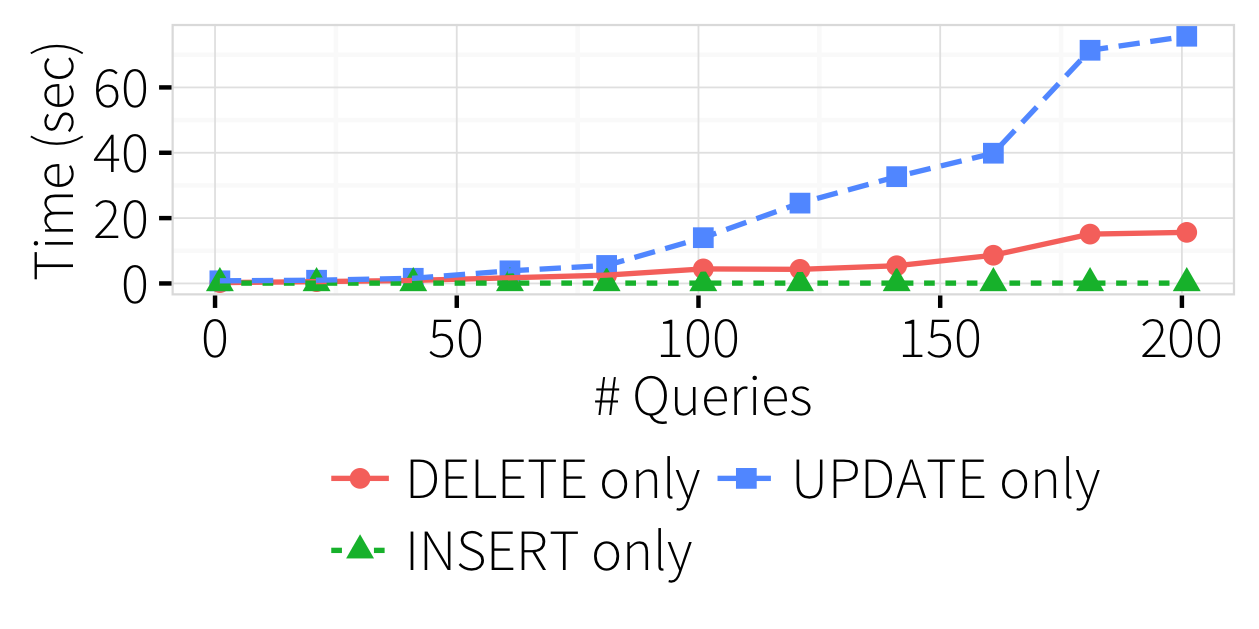
\includegraphics[width = .99\columnwidth]{figures/indelup_time}
      \caption{Performance for different query types.}
      \label{f:indelup_time} 
    \end{subfigure}
    \begin{subfigure}[t]{.33\textwidth}
      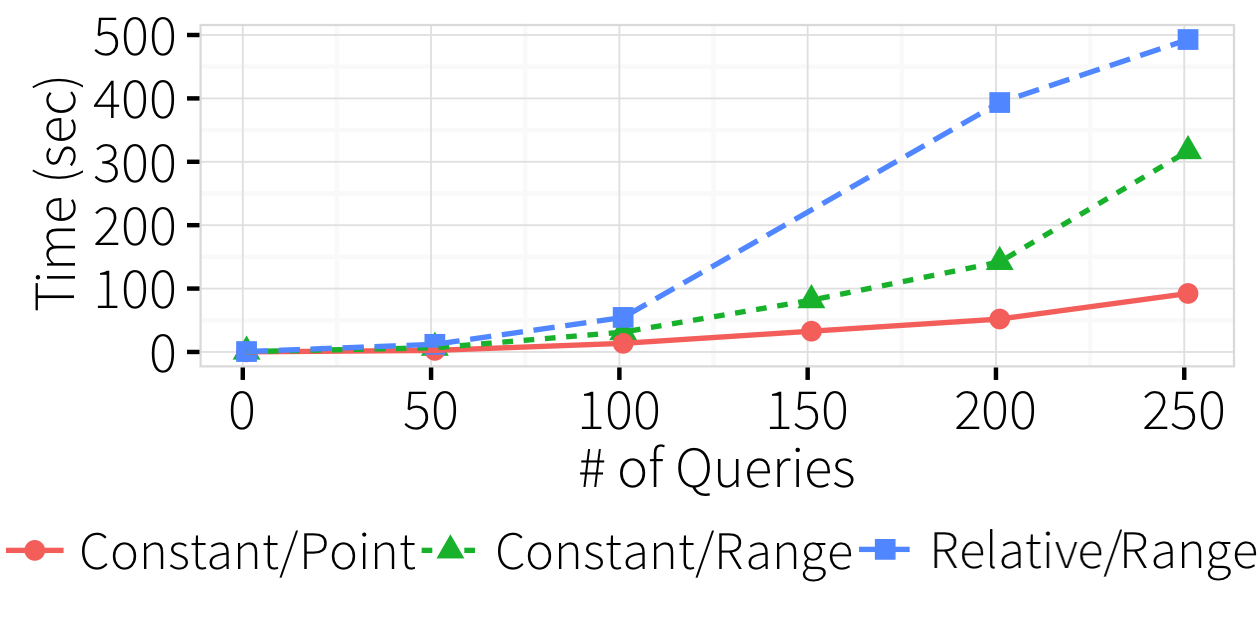
\includegraphics[width = .99\columnwidth]{figures/pointrelv_time}
      \caption{Performance of diff. query clause types.}
      \label{f:qidx_time} 
    \end{subfigure}
    \begin{subfigure}[t]{.33\textwidth}
      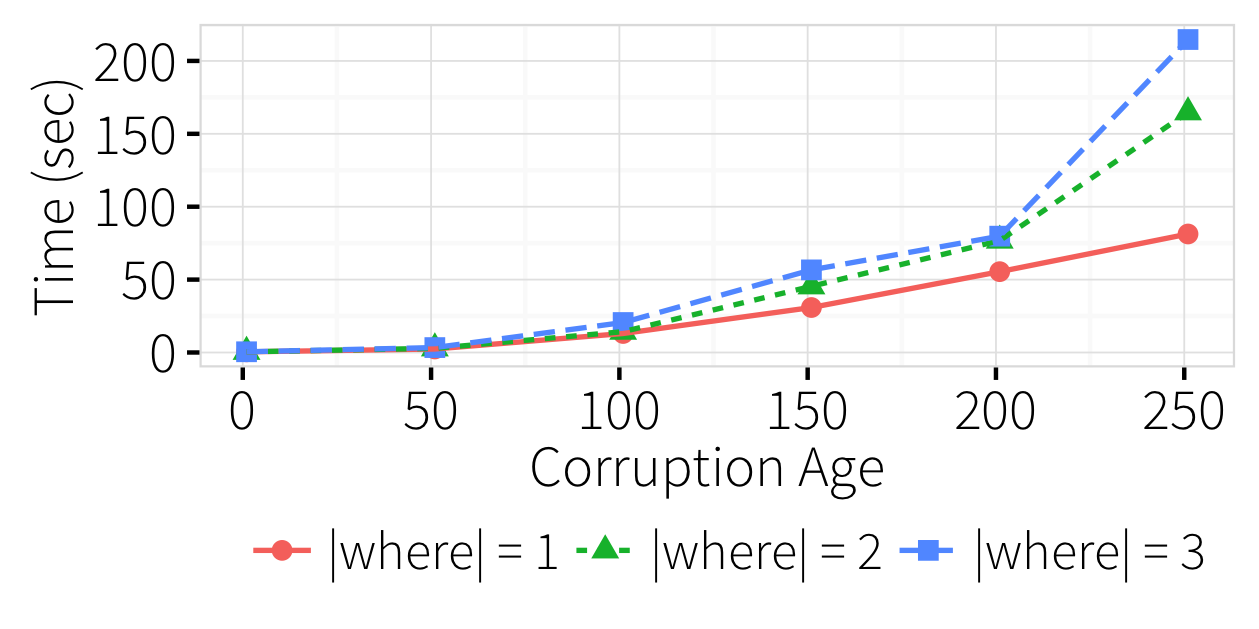
\includegraphics[width = .99\columnwidth]{figures/where_time}
      \caption{Query dimensionality vs time.}
      \label{f:where_time} 
    \end{subfigure}
    \caption{ \sys can repair \texttt{INSERT} and \texttt{DELETE} workloads quickly; complex \texttt{UPDATE} queries are more expensive to repair.}
  \end{figure*}
 



\stitle{Synthetic:} \label{sec:syntheticgen}
We generate an initial database of $N_D$ random tuples.  
The schema contains a primary key $id$ along with $N_a$ attributes $a_1\ldots a_{N_a}$, whose values are integers picked from $[0, V_d]$ uniformly at random.
We then generate a sequence of $N_q$ queries. 
The default setting for these parameters are: $N_D = 1000, N_a = 10, V_d = 200, N_q = 300$. 


\texttt{UPDATE} queries are defined by a SET clause that assigns an attribute a $Constant$ or $Relative$ value,
and a WHERE clause can either be a $Point$ predicate on a key, or a $Range$ predicate on non-key attributes:

\begin{scriptsize}
\begin{verbatim}
 SET Clause:                WHERE Clause:
  Constant: SET (a_i=?), ..   Point: WHERE a_j=? & ..
  Relative: SET (a_i=a_i+?)   Range: WHERE a_j in [?,?+r] & ..\end{verbatim}
\end{scriptsize}
\noindent where \verb|?|$\in [0, V_d]$ is random and \verb|r| is the size of the range predicate. 
Query selectivity is by default $2\%$ (\verb|r|$=4$).
Note that a range predicate where \texttt{r = 0} is distinct from a $Point$ predicate due to the non-key attribute.
The WHERE clauses in \texttt{DELETE} queries are generated in an identical fashion, while
\texttt{INSERT} queries insert values picked uniformly at random from $V_d$.
By default, we generate \texttt{UPDATE} queries with non-key range predicates and constant set clauses.
  
% In addition, the skew parameter $s$ determines the distribution attributes referenced in the \texttt{WHERE} and \texttt{SET} clauses.  
% Each attribute in a query is picked from either a uniform distribution when $s=0$ or a zipfian distribution with exponent $s$.
% This allows our experiments to vary between a uniform distribution, where each attribute is
% equally likely to be picked, and a skewed distribution where nearly all attributes are the same. 


\looseness -1
\stitle{Benchmarks: } We use the TPC-C~\cite{tpcc} and TATP~\cite{tatp} benchmarks.
The former generates the {\it ORDER} table at scale 1 with one warehouse, and uses the queries that modify the {\it ORDER} table. 
We execute a log of $2000$ queries over an initial table containing 6000 tuples.  
$1837$ queries are \texttt{INSERT}s and the rest are \texttt{UPDATE}s. 
The latter TATP workload simulates the caller location system. 
We generate a database from {\it SUBSCRIBER} table with 5000 tuples and $2000$ \texttt{UPDATE} queries.
Both setups were generated using the OLTP-bench~\cite{difallah2013oltp}. 



\stitle{Corrupting Queries:} We corrupt query $q_i$ by replacing it with a randomly
generated query of the same type based on the procedures described above.
To standardize our procedures, we selected a fixed set of queries indexes based on their age with respect to the most recent query.
For instance, an age of $50$ means the corruption was $50$ queries ago on $q_{N_q-50}$.
We call this parameter the {\it Corruption Age}.

%\xlw{We finally introduce the query corruption(s) at multiple query indexes $q_{N-idx}, idx \in [50, 300]$. We denote the number of queries executed after the first corruption as $N_{Q}$ ($\#\ of\ Queries$), $N_{Q} = N-idx$ and it measures the hardness of the synthetic problem.} 


\subsection{Benchmarks}
\label{sec:experiments:benchmark}
In this experiment, we vary the location of a single corrupt query in the TPC-C and TATP benchmark query logs and report \sys's performance;
in all runs, \sys achieves an F1 score of $1$.
Figure~\ref{f:tpcctatp} shows that \sys can generate a repair for TPC-C and TATP within milliseconds and tens of seconds, respectively.
The key reason is that in practice, each query affects a small set of records and results in a very small complaint set---$1-2$ on average.
Tuple and query slicing are also able to aggressively reduce the total number of constraints to $<100$ constraints on average.

\sys can repair TPC-C  queries are predominantly \texttt{INSERT}s, which \sys can solve within milliseconds. 
In contraist, TATP only contains \texttt{UPDATE}s, which are harder to solve than \texttt{INSERT} queries and thus lead to higher execution time compared with TPC-C queries.
Note that these experiments stripped out read-only queries from the workload, which account for $8$ and $80\%$ of the queries in TPC-C and TATP, respectively.
Finally, \sys repairs Example~\ref{ex:taxes} in Figure~\ref{fig:example} within 35 milliseconds. 

\begin{figure}[h]
\centering
  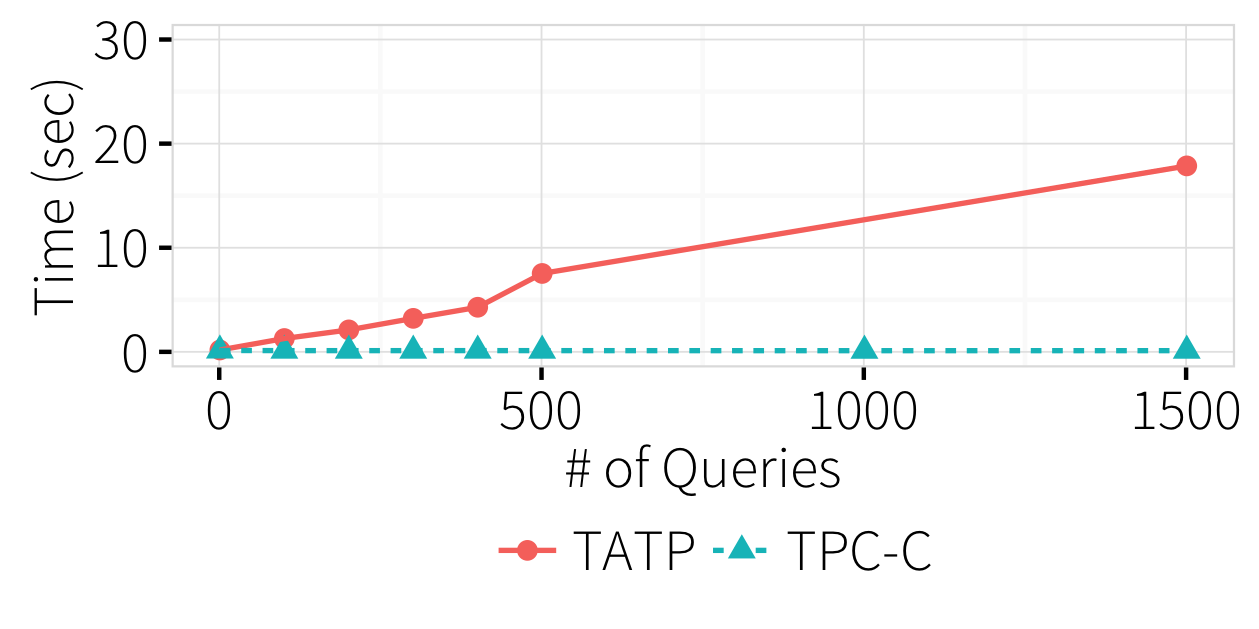
\includegraphics[width = .75\columnwidth]{figures/benchmark_time}
  \vspace*{-.2in}
  \caption{\sys quickly produces repairs for OLTP workloads.}
  \label{f:tpcctatp} 
\end{figure}

{\it Takeaways: many workloads in practice are dominated by \texttt{INSERT} and point \texttt{UPDATE} queries (ignoring the dominant percentage of read-only queries).  
In these settings, \sys is very effective at reducing the number of constraints and can derive repairs with near-interactive latencies.}

 \begin{figure*}[!htb]
    \vspace*{-.1in}
    \centering
    \begin{subfigure}[t]{.49\textwidth}
    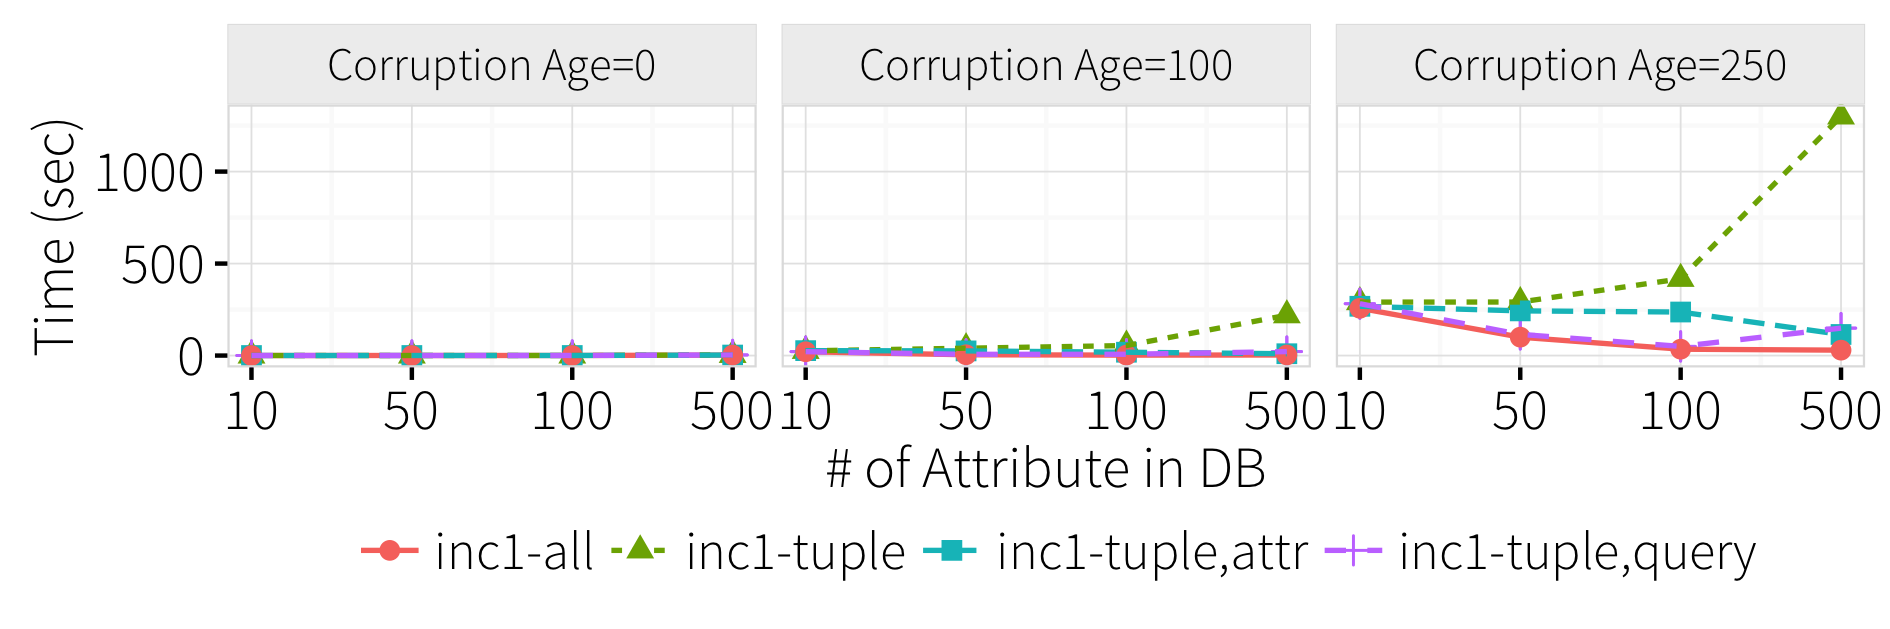
\includegraphics[width = .99\columnwidth]{figures/attr_time}
    \vspace*{-.1in}
    \caption{\# of attributes vs time ($N_D = 100$).}
    \label{f:attr} 
    \end{subfigure}
    \begin{subfigure}[t]{.49\textwidth}
    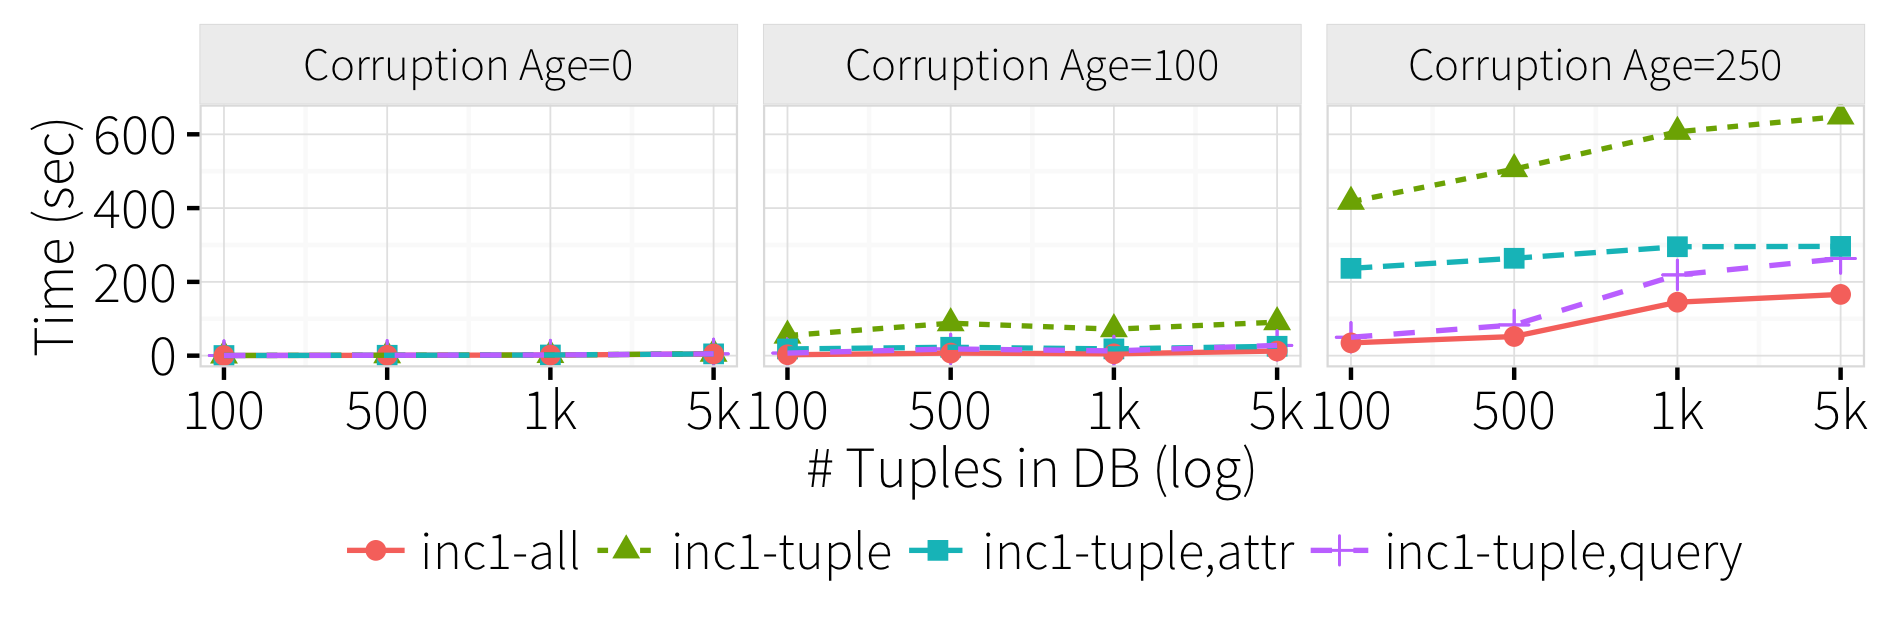
\includegraphics[width = .99\columnwidth]{figures/attr100_time}
    \vspace*{-.1in}
    \caption{Database size vs time ($N_a = 100$).}
    \label{f:attr100} 
    \end{subfigure}
    \vspace*{-.1in}
    \caption{For datasets with many attributes or many records, the optimizations result in significant improvements.}
    \label{f:database}
  \end{figure*}

\subsection{Sensitivity of the Incremental Algorithms}
\label{sec:experiments:inc}


This subsection evaluates the efficacy of using each slicing optimization on the incremental algorithm by varying the characteristics of the database and query log.  
By default, the tuple-slicing optimization is always enabled because the algorithms are unable to scale beyond $50$ queries without it (Figure~\ref{fig:querysize_vs_time}).
We report performance and omit accuracy numbers because the F1 for all settings is nearly 1.


\subsubsection{Sensitivity to the Query Log}
\label{sec:experiments:synth}

The following experiments evaluate \sys (incremental with all optimizations) under differing query log characteristics.
We first vary the query type and find that \texttt{UPDATE} queries are the most expensive query type to repair.
We then focus solely on \texttt{UPDATE}-only workloads and vary query complexity and predicate dimensionality.
The database is set to the default settings ($N_a=10$, $N_D=1000$, $N_q=300$) and we vary the location of the single corrupt query.
%\xlw{and we adjust the query corruption from $q_N$ to $q_{N-250}$ ($\#\ of\ Queries$ vary from $0$ to $250$). }

\stitle{Query Type: }\label{sec:indelup}
This experiment compares \sys over \texttt{INSERT}, \texttt{DELETE}, or \texttt{UPDATE}-only query logs to test the effect of the query type.
Figure~\ref{f:indelup_time} shows that while the cost of repairing \texttt{INSERT} workloads
remains relatively constant, the cost for \texttt{DELETE}-only and \texttt{UPDATE}-only workloads increase as 
the corruption happens earlier in the query log---and a much faster rate for \texttt{UPDATE} queries.
This is because \texttt{UPDATE} queries translate into more undetermined variables than \texttt{INSERT} or \texttt{DELETE} queries, and are significantly more expensive to repair. 
For this reason, our subsequent experiments focus specifically on the more challenging \texttt{UPDATE}-only workloads.

\smallskip
\stitle{Query Clause Type: }
So far, we have focused on \texttt{UPDATE} queries with constant set clauses and range predicates ({\it Constant/Range}).  
Figure~\ref{f:qidx_time} compares this against {\it Constant/Point} and {\it Relative/Range} \texttt{UPDATE} query workloads. 
%\ewu{Is this true:} The x-axis varies the number of queries from $0$ to $250$.
We found that point predicates are easier to solve than range predicates because 
1) the latter doubles the number of undetermined variables as compared to point predicates and 
2) point queries are on key attributes, which further reduces the MILP search space.
In addition, constant set clauses are easier than relative set clauses because
We believe constant set clauses are simpler than relative set clauses  because the former breaks the causal relationship between input and output records for the overwritten values.
This both simplifies the difficulty of the constraint problem, and reduces the total number of constraints.


\smallskip
\stitle{Predicate Dimensionality:}
Figure~\ref{f:where_time} varies the dimensionality of the update queries by increasing the number of predicates in the \texttt{WHERE} clause, while keeping the query cardinality constant (so the number of complaints is fixed).
The cost increases with the dimensionality because each additional predicate is translated into a new set of constraints and undetermined variables, increasing the problem complexity.
% We note that many OLTP queries primarily involve key predicates and low dimensional predicates.

\smallskip
\textit{
  Takeaways: we find \texttt{UPDATE}-workloads are on average significantly harder than workloads with other types of queries, and that
  performance is closely related to the complexity and the dimensionality of queries. 
  In the challenging setting of range \texttt{UPDATE}-only workloads, \sys find a repair within seconds or minutes for ~$200$ queries---particularly if the corruption is recent. 
}




\subsubsection{Sensitivity to Database Properties}
\label{sec:experiments:dbproperties}

The following two experiments compare different combinations of the slicing optimizations \emph{tuple/query/attr} under varying database size and schema size settings.  
The query log contains the default $N_q = 300$ {\it Constant/Range} \texttt{UPDATE} queries.
Each facet (subplot) in Figure~\ref{f:database} represents the location of the corruption as $q_{N_q-250}, q_{N_q-100}, q_{N_q-0}$.

\stitle{\# of Attribute:} \looseness -1
We first vary the number of attribute ($N_a \in [10, 500]$) under a fixed database size $N_D = 100$.
As shown in Figure~\ref{f:attr}, when the number of attribute in a table is small (e.g., $N_a=10$) or when the corruption is recent (e.g., $q_{200, 300}$), then all optimizations appear identical. 
However, increasing the number of attribute exhibits a larger benefit for query and attribute slicing (up to $6.8\times$ reduction compared to tuple-slicing).
When the table is wide ($N_a = 500$), applying all optimizations ($inc_1-all$) is $40\times$ faster than tuple-slicing alone.  


\stitle{Database Size:} \looseness -1
We now vary the database size ($N_D \in [100,5000]$) with a large number of attributes ($N_a = 100$).
We fix the number of complaints by decreasing the query selectivity in proportion to $N_D$'s increase---the specific mechanism to do so did not affect the findings.
Figure~\ref{f:attr100} shows that the costs are relatively flat until the corruption occurs in an old query ($Corruption\ Age = 250$).  
In addition, we find that the cost is highly correlated with the number of candidate queries that are encoded in the MILP problem.
The increase in cost despite tuple-slicing is due to the increasing number of candidate queries in the system; 
we believe this increasing trend is due to the solver's ability to prune constraints that correspond to queries that clearly will not affect the complaint set---an implicit form of query slicing.  
Applying attribute-slicing supercedes this implicit optimization and results in a flat curve, 
while query-slicing explicitly reduces the number of candidate queries in proportion with the database size, and leads to the increasing trend.
Ultimately, combining all three optimizations outperforms tuple-slicing by $2-4\times$.

\smallskip
\textit{
  Takeaways: we find that repair performance is sensitive to 
  the number of attributes and the number of tuples in the database, particularly when the corruption is old. 
  Tuple slicing is essential to solve general problems, while attribute and query slicing show significant gain for datasets with large number of attributes.
}



\subsection{More Challenging Repair Settings}
\label{sec:experiments:hardprob}

In this section, we further study the performance of \sys in solving hard problems---when the set of complaints is incomplete, and when there is more than one corruption that let to the complaints\footnote{
\footnotesize Note that even when there are multiple corruptions in the log, the incremental algorithm is still applicable if only one is responsible for the set of complaints.}.
 
\stitle{Incomplete Complaint Set:} \looseness -1
The first experiment (Figures~\ref{f:falsenegative_time} and~\ref{f:falsenegative_acc}) varies the fase positive rate in incomplete complaint sets.
We increase the rate from $0$ ($0\%$ missing in the complaint set) to $.75$ ($75\%$ are missing).  
We find that reducing the size of the submitted complaint set naturally improves the repair performance,
however the repair quality  (precision and recall in Figure~\ref{f:falsenegative_acc}) may suffer if the corruption occured in a very old query. 
This is expected because \sys targets reported complaints, thus unreported complaints may be missed and lead to low recall.
Also, despite tuple-slicing's refinement step, the repair may over generalize and ``fix'' the wrong records, leading to low precision.


    
\begin{figure}[!htb]
  \hspace*{-.1in}
  \centering
    \begin{subfigure}[t]{.33\textwidth}
      %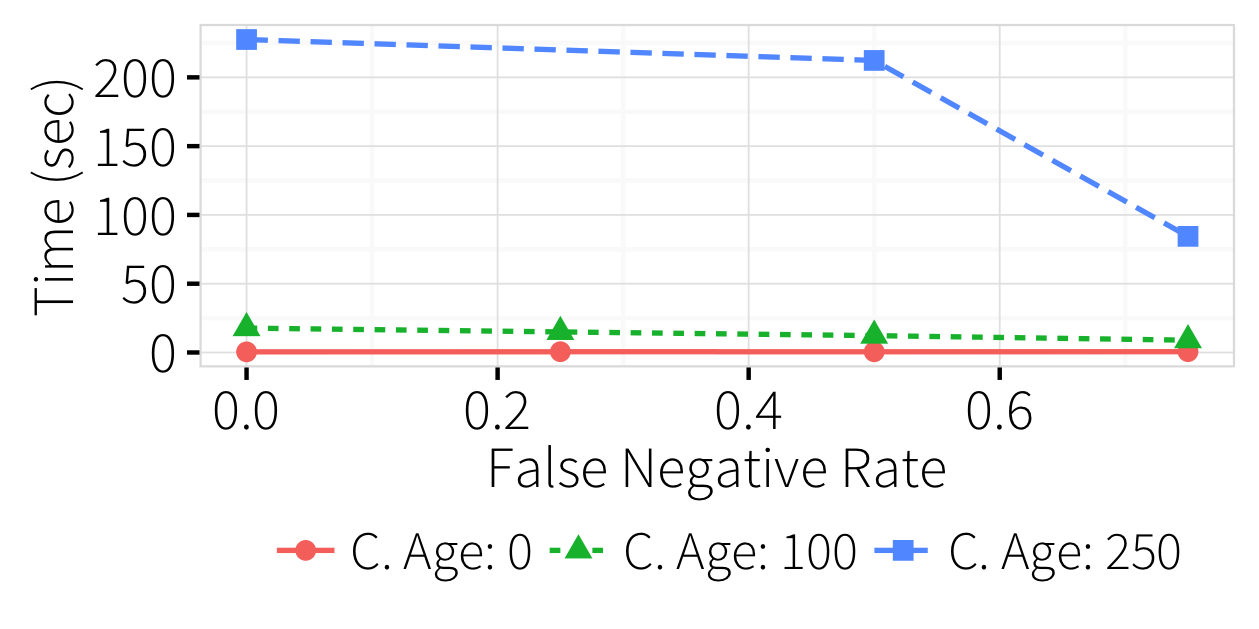
\includegraphics[width = .99\columnwidth]{figures/noise_fn_time} 
      % or full label in 2 lines
      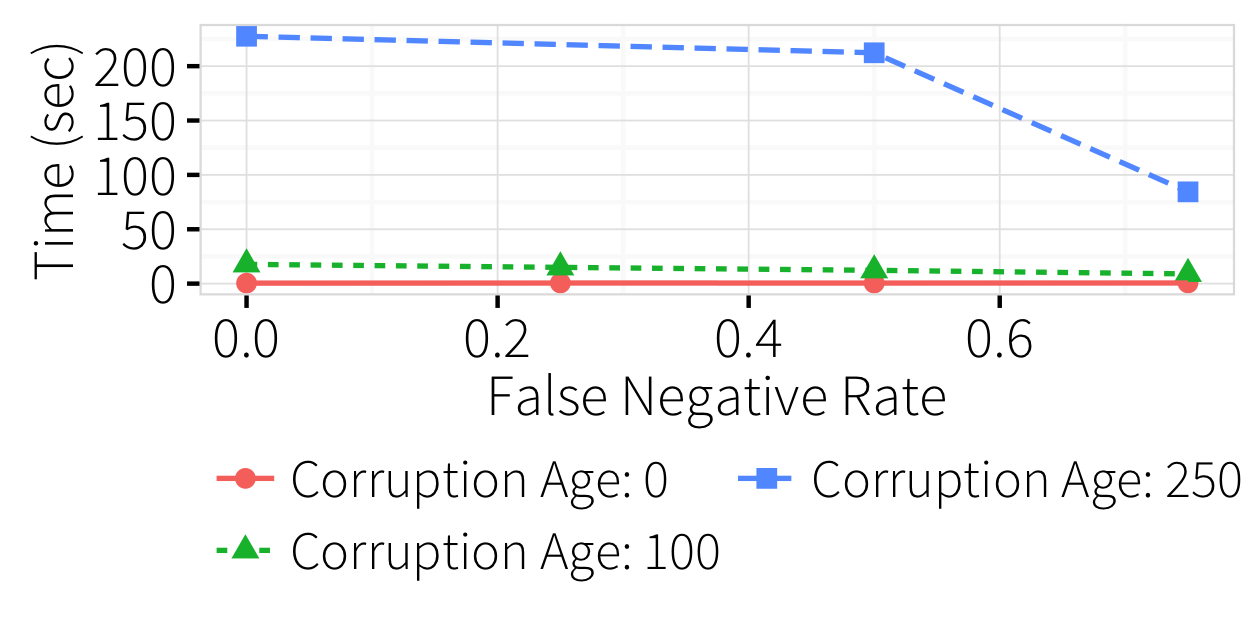
\includegraphics[width = .99\columnwidth]{figures/noise_fn_time_fulllabel} 
      \vspace*{-.1in}
      \caption{False negatives vs time.}
      \label{f:falsenegative_time} 
    \end{subfigure}
    \\
    \begin{subfigure}[t]{.33\textwidth}
      %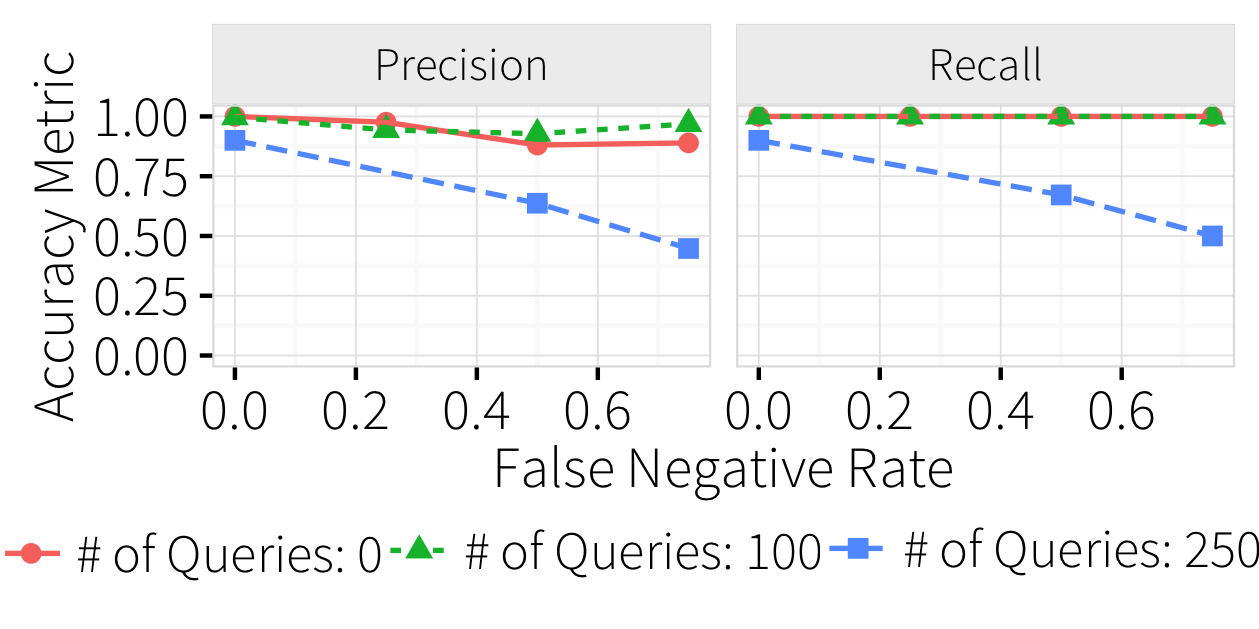
\includegraphics[width = .99\columnwidth]{figures/noise_fn_acc}
      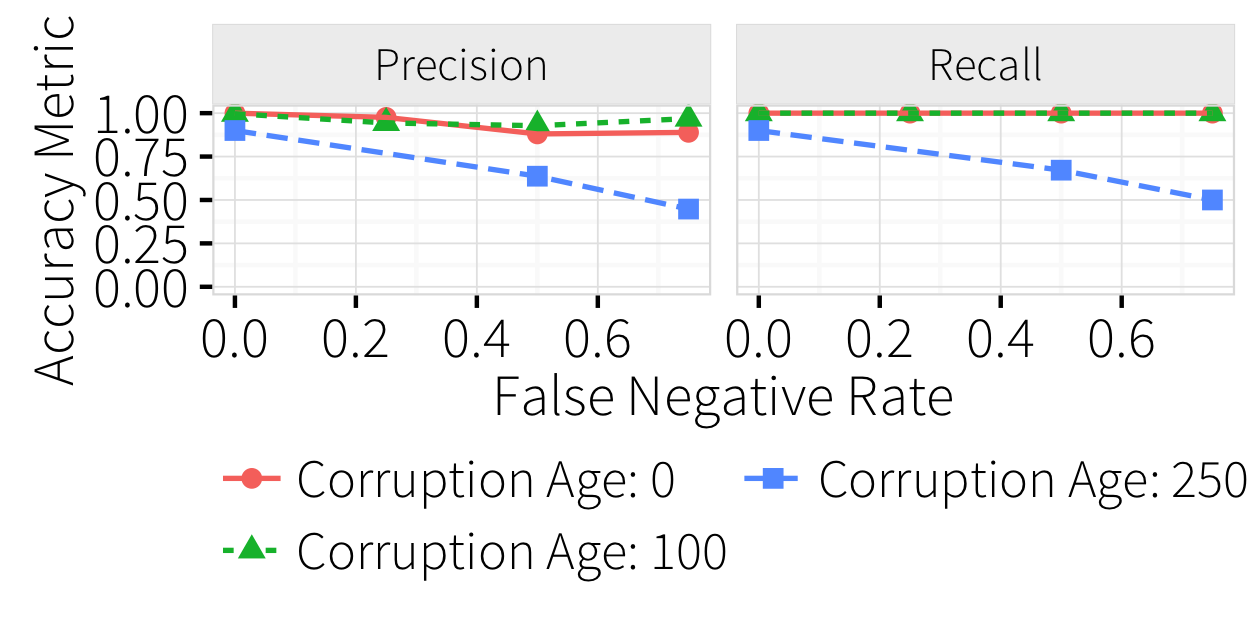
\includegraphics[width = .99\columnwidth]{figures/noise_fn_acc_fulllabel}
      \vspace*{-.1in}
      \caption{False negatives vs accuracy.}
      \label{f:falsenegative_acc} 
    \end{subfigure}
    \vspace*{-.1in}
    \caption{Incomplete complaint sets improve repair speed due to less complaints, but degrade repair quality for older corruption. }
  \end{figure}



\stitle{Multiple Corrupt Queries:} \looseness -1
This experiment studies how the \naive algorithm, along with the slicing optimizations, are able to repair complaints resulting from multiple corrupt queries.
We use the default settings, vary the number of corruptions using the following procedure:
we  corrupt every tenth query in the log starting from oldest query $q_1$, and vary the \texttt{UPDATE}-only query log size  in increments of $10$ within $[10, 50]$ inclusive.
%$N_q\in \{10, 20, 30, 40, 50\}$, and
For example, when the $N_q = {30}$, we corrupt queries $q_{1,11,21}$. 

We find that all variants of \naive have difficulty scaling beyond $30$ queries (consistent with the case with one corrupt query in Figure~\ref{fig:querysize_vs_time}), although tuple and query slicing modestly improve repair performance and quality.
In addition, the number of corruptions and queries greatly affect the scalabality (Figure~\ref{f:multi_time}) and the accuracy (Figure~\ref{f:multi_acc}) of the algorithms. 
Specifically, as the corruptions increase, the number of possible assignments of the MILP parameters increases exponentially and the solver often takes longer than our experimental time limit of $1000$ seconds and returns an empty result.
We find that problem infeasibility is the predominant explanation for why the accuracy degrades past $30$ queries.  
For example, with $40$ queries ($4$ corruptions), \naive takes nearly $750$s; however if we ignore the infeasible executions, the average is $300$ seconds and the precision and recall are greater than $0.94$.  
Unfortunately, with $50$ queries ($5$ corruptions), all runs are infeasible and exceed the time limit.

  \begin{figure}[!htb]
  \hspace*{-.1in}
  \centering
    \vspace*{-.2in}
    \begin{subfigure}[t]{.33\textwidth}
    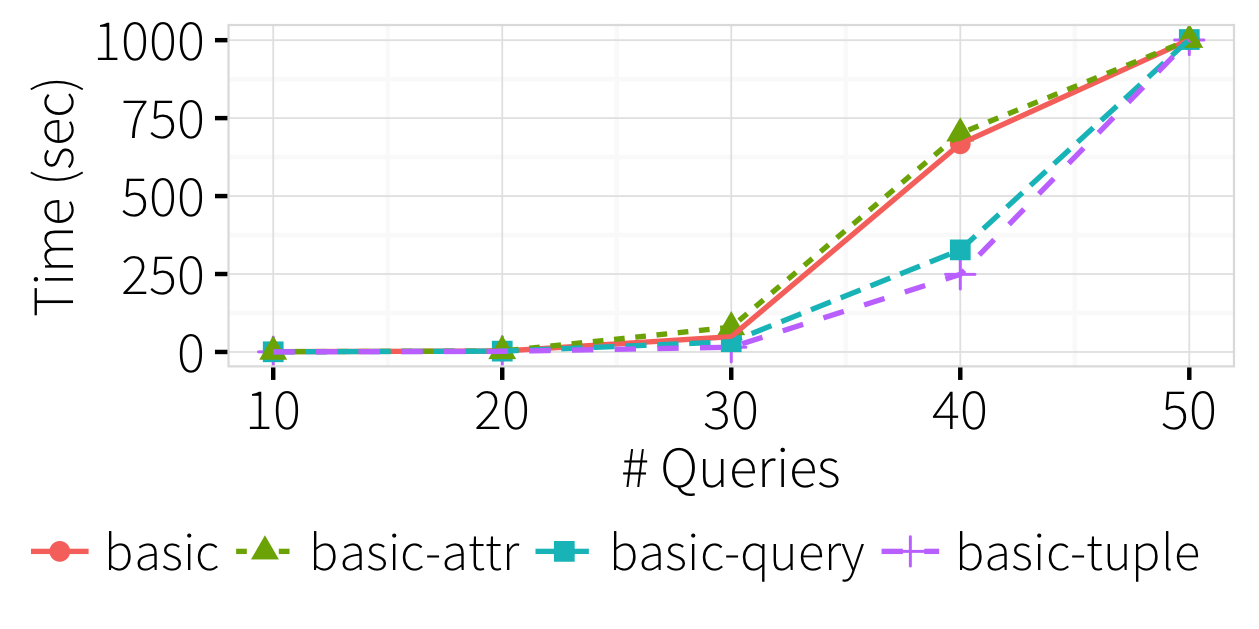
\includegraphics[width = .99\columnwidth]{figures/multi_time}
    \caption{Performance for multiple corruptions.}
    \label{f:multi_time} 
    \end{subfigure}
    \\
        \begin{subfigure}[t]{.33\textwidth}
    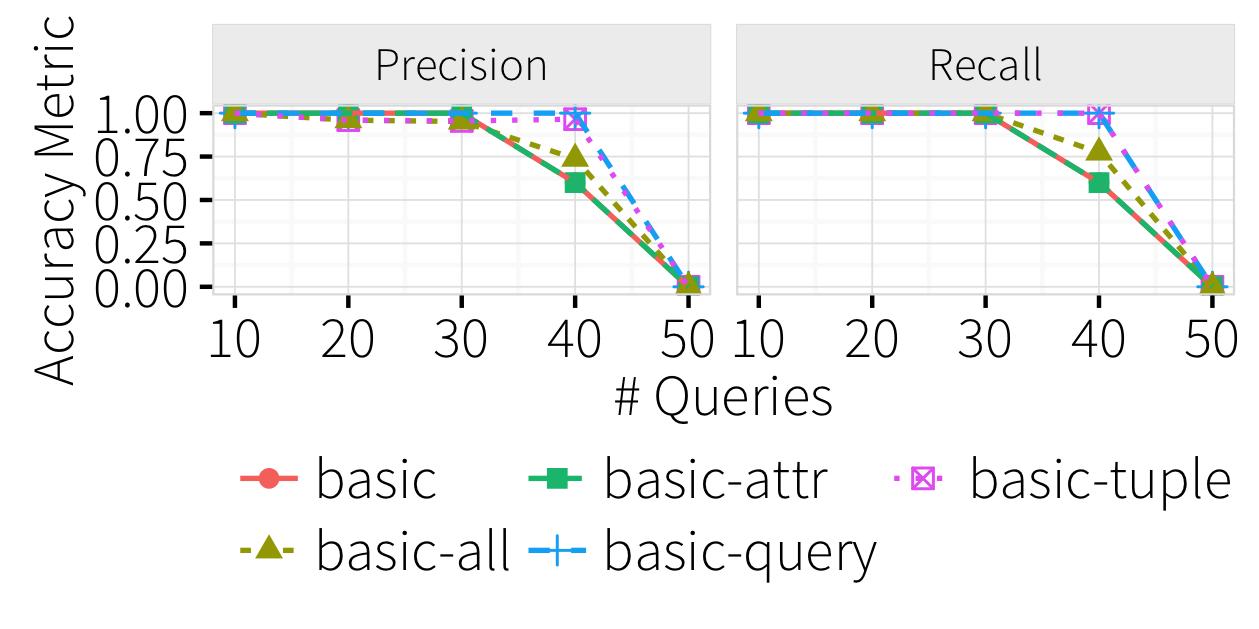
\includegraphics[width = .99\columnwidth]{figures/multi_pr}
    \caption{Accuracy for multiple corruptions.}
    \label{f:multi_acc} 
    \end{subfigure}
        \vspace*{-.1in}
    \caption{Our analysis highlights limitations of \naive, the value of tuple-slicing, and the high cost of \texttt{UPDATE} queries.}
  \end{figure}



\smallskip
\emph{
Takeaways: \sys solves recent errors (e.g., errors in most recent 100 queries) efficiently and effectively even with very incomplete complaint information. 
Also, \naive, even with slicing optimizations, has severe scalability limitations due to the large number of undetermined variables---this is unsurprising as MILP constraint solving is an NP-hard problem.
This result highlights the value of the incremental algorithm optimization.
}


\iffalse
\emph{Skew:} We now study the effects of attribute skew on the algorithms.
We increase the skew parameter from $0$ (uniform) to $1$ (nearly every attribute is $A_0$) 
and find a reduction in latency (Figure~\ref{f:skew_time}).
We believe the reason is because increasing the skew focuses the query predicates over a smaller set of logical attributes, 
and increases the number of constraints placed on each of the logical attributes used in the query log.  
Each of these constraints reduces the search space of allowable values for that attribute, and thus simplifies the MILP problem.
This result suggests that \sys may be well suited for many transaction systems that naturally exhibit query skew.
Note that the overall number of constraints in the problem is the same, only their distribution over the query attributes has changed.

\stitle{Single Corrupt Query:}
In this experiment, we evaluate the efficacy \sys with tuple slicing and incremental optimization
in the special case when one query has been corrupted in a much larger query log. 
We compare \incremental without tuple slicing ($inc_1$) against tuple slicing at 
different batching levels of 1, 2, 8 ($inc_1-tuple; inc_2-tuple, inc_8-tuple$). 
Recall from Section~\ref{sec:incremental} that $inc_k$ parameterizes $k$ consecutive queries in each batch until a repair is found.
Figure~\ref{f:singlequeryinc_time} highlights the scalability limitation of the incremental 
algorithm without tuple-slicing: with 50 queries $inc_1$  easily exceeds the 1000s limit.   
The tuple-slicing scales significantly better (nearly $200\times$ faster), however
the accuracy severely degrades when $k>1$.  
The primary reason is because of infeasibility errors---the MILP problem is much harder, and fails to find a repair.  
This is highlighted by the symmetry between the precision and recall curves.  
A secondary reason is beause the refinement step of  tuple slicing may not generate a fully correct repair and generalize incorrectly.
This is why the precision curve is lower than the recall curve for $inc_8-tuple$.
\fi


